% Provenance (never printed): see sources/outline_sources.md (Year 2: mid-latitude cyclones and
% fronts; jets and Rossby waves, descriptive; tropical cyclones; numerical weather prediction,
% principle). Definitions after the NWS glossary and UCAR; cyclogenesis conditions after the NOAA
% AOML FAQ; potential intensity after Gilford (2021, pyPI); conveyor belts after Raveh-Rubin and
% Catto (2019); blocking after Wang and others (2026); predictability after Krishnamurthy (2019),
% Selz and others (2022) and ECMWF. The Lorenz system from figdata/bachelor-2/weather.py; the
% fronts, waves and storms of the examples, exercises and problem are invented, their values
% computed in the Book 4 scratch calculator calc/ch22.py.
\chapter{Weersystemen}\label{ch:b2:weather-systems}

Een verwachting voor vier dagen vooruit is nu even nauwkeurig als een verwachting voor één dag vooruit dertig
jaar geleden was, en elk decennium heeft ongeveer een dag bruikbare verwachting toegevoegd. Toch is geen verwachting van het
weer op een bepaalde dag, op een bepaalde plaats, betrouwbaar veel verder dan tien dagen, en betere computers
alleen zullen die grens niet ver opschuiven: de atmosfeer versterkt haar eigen kleine onzekerheden. Dit
hoofdstuk beschrijft de weersystemen die verwachtingen volgen, de fronten en depressies van de
middelbare breedten, de golven van de straalstroom en de tropische cyclonen, en daarna de manier waarop ze
worden verwacht en waarom de verwachting ergens moet ophouden.
% ledger: mo:accuracy, bauer:day-per-decade, krish19:predictability

\begin{recall}
\textbf{Uit de schoolboeken}: luchtmassa's, fronten, koufronten en warmtefronten, depressies en
anticyclonen, isobaren en weersverwachtingen; de tropische cycloon, zijn oog en oogwand, de
schaal van Saffir--Simpson. \textbf{Uit Boek~3}: de drukgradiëntkracht, de
Coriolisparameter $f = 2\Omega\sin\varphi$, geostrofisch evenwicht, cyclonen en anticyclonen, de
drie cellen, de westenwinden en de straalstromen. \textbf{Uit de natuurkundeboeken}: warmtemotoren
en het rendement van een carnotcyclus. \textbf{Uit \cref{ch:b2:atmospheric-thermodynamics}}:
verzadiging, de \omterm{def:b2:atmospheric-thermodynamics:moist-adiabat}{natte adiabaat}, $\theta_e$, \omterm{def:b2:atmospheric-thermodynamics:instability}{voorwaardelijke instabiliteit} en CAPE.
\end{recall}

\section{Fronten}\label{sec:b2:weather-systems:fronts}

De schoolboeken tekenden fronten als lijnen op een kaart. Een front is de lijn waar een hellende grens
tussen twee luchtmassa's de grond raakt, en zijn weer komt van die helling.

\begin{definition}[Frontvlak; stationair front; occlusiefront]\label{def:b2:weather-systems:fronts}
Het \emph{frontvlak}\index{frontvlak} van een front is de hellende grens tussen
de twee luchtmassa's, waarbij de dichtere, koudere als een wig onder ligt; het front op de kaart is zijn
snijlijn met de grond. Een \emph{stationair front}\index{stationair front} is een front
dat heel traag of helemaal niet beweegt. Een \emph{occlusiefront}\index{occlusiefront} is een
samenstelling van twee fronten, ontstaan wanneer een koufront een warmtefront of stationair front inhaalt.
\end{definition}
% ledger: nws4:front, nws4:stationary, nws4:occluded

Een \omterm{def:b2:weather-systems:fronts}{stationair front} ontstaat wanneer geen van beide luchtmassa's de andere kan wegduwen, en de winden langs het
front waaien in plaats van eroverheen; het kan dagen blijven liggen, bewolkt en nat, voordat het weer als koufront
of als warmtefront gaat bewegen. Op een kaart wisselt het de blauwe driehoeken van een koufront, die naar de
warme lucht wijzen, af met de rode halve cirkels van een warmtefront, die naar de koude lucht wijzen. Een
\omterm{def:b2:weather-systems:fronts}{occlusiefront} wordt in paars getekend, met beide symbolen aan dezelfde kant. Wanneer de lucht achter het koufront
de koudste is, schuift ze onder het warmtefront en tilt het omhoog, een koude occlusie; wanneer de lucht
vóór het warmtefront de koudste is, glijdt het koufront eroverheen omhoog, een warme occlusie.
% ledger: ucar4:stationary-occluded, nws4:occluded

Hoe steil is een \omterm{def:b2:weather-systems:fronts}{frontvlak}? Het antwoord verbindt het hydrostatisch evenwicht met het geostrofisch
evenwicht uit Boek~3.

\begin{proposition}[Helling van een frontvlak]\label{prop:b2:weather-systems:slope}
Laat een \omterm{def:b2:weather-systems:fronts}{frontvlak} koude lucht met de temperatuur $T_c$ scheiden van warme lucht met $T_w$, met
geostrofische winden $v_c$ en $v_w$ langs het front. Neem de as $x$ dwars op het front naar de
koude lucht en de as $y$ erlangs, zodat $(x, y, z)$ rechtshandig is. Dan stijgt het
\omterm{def:b2:weather-systems:fronts}{frontvlak} naar de koude lucht toe met de helling
\[
  \tan\alpha \approx \frac{f\,\bar T\,(v_c - v_w)}{g\,(T_w - T_c)},
\]
waarin $\bar T$ de gemiddelde temperatuur is. Een \omterm{def:b2:weather-systems:fronts}{frontvlak} in evenwicht vereist een sprong van de wind
erlangs, $v_c > v_w$: de wind draait cyclonaal over het front.
\end{proposition}

\begin{proof}
De druk is continu over het \omterm{def:b2:weather-systems:fronts}{frontvlak}, dus zijn verandering langs het vlak is
dezelfde, aan welke kant ze ook wordt berekend: $\partial_x p_c\,\mathrm{d}x + \partial_z p_c\,\mathrm{d}z =
\partial_x p_w\,\mathrm{d}x + \partial_z p_w\,\mathrm{d}z$. Aan elke kant is $\partial_z p = -\rho g$
(hydrostatisch evenwicht) en $\partial_x p = \rho f v$ (geostrofisch evenwicht). Dus
$\rho_c f v_c\,\mathrm{d}x - \rho_c g\,\mathrm{d}z = \rho_w f v_w\,\mathrm{d}x - \rho_w
g\,\mathrm{d}z$, en
\[
  \frac{\mathrm{d}z}{\mathrm{d}x} = \frac{f(\rho_c v_c - \rho_w v_w)}{g(\rho_c - \rho_w)} .
\]
Bij dezelfde druk is $\rho \propto 1/T$, dus $\rho_c - \rho_w \approx \bar\rho\,(T_w -
T_c)/\bar T$; in de teller kan het kleine verschil van de dichtheden worden verwaarloosd, wat
de formule geeft. De koude lucht ligt onder, dus het vlak stijgt naar haar toe, $\mathrm{d}z/
\mathrm{d}x > 0$, en $v_c > v_w$. Met $x$ naar de koude lucht is de relatieve vorticiteit
$\partial v/\partial x$ over het front dan positief: cyclonaal.
\end{proof}

\begin{example}[Een typische helling]\label{ex:b2:weather-systems:slope}
Op \ang{45}~NB is $f = \qty{1.03e-4}{s^{-1}}$. Over een front met $\bar T = \qty{280}{K}$, een
temperatuurcontrast van \qty{5}{K} en een wind die erlangs met \qty{10}{m/s} verandert, is $\tan\alpha
= 1.03 \times 10^{-4} \times 280 \times 10/(9.81 \times 5) = 0.0059$, ongeveer 1 op 170: het
\omterm{def:b2:weather-systems:fronts}{frontvlak} bereikt een hoogte van \qty{1}{km} zo'n \qty{170}{km} van het front aan de grond.
Een scherpere windsprong geeft een steiler vlak; een sterker temperatuurcontrast, een vlakker.
\end{example}

Echte fronten hebben hellingen van deze orde, en de ondiepe wig verklaart hun weer. Vóór een
warmtefront glijdt de warme lucht honderden kilometers lang over een flauwe helling omhoog: hoge wolken,
cirrus en cirrostratus, komen eerst, dan altostratus, en de wolken worden dikker en lager tot
de regen dicht bij het front inzet. Een koufront, steiler en sneller, tot twee keer zo snel als een
warmtefront, tilt de warme lucht abrupt op: cumulus en cumulonimbus, buien, windstoten en een plotselinge daling
van de temperatuur, met een druk die ophoudt met dalen en begint te stijgen terwijl het front passeert. Een front
waar de warme lucht langs het \omterm{def:b2:weather-systems:fronts}{frontvlak} daalt in plaats van erlangs te stijgen, heet een katafront.
% ledger: ucar:warm-front, ucar:cold-front, nws4:front

\begin{omfigure}
\centering
\begin{tikzpicture}[font=\scriptsize, >=Stealth, x=1cm, y=1cm]
% air masses
\fill[omCold!12] (0,0) -- (0,3.4) .. controls (1.6,2.2) and (3.2,0.8) .. (4,0) -- cycle;
\fill[omCold!12] (9.6,0) .. controls (11,0.6) and (12.6,1.5) .. (14,2.4) -- (14,0) -- cycle;
\fill[omWarm!8] (4,0) .. controls (3.2,0.8) and (1.6,2.2) .. (0,3.4) -- (0,4.8) -- (14,4.8)
  -- (14,2.4) .. controls (12.6,1.5) and (11,0.6) .. (9.6,0) -- cycle;
% frontal surfaces
\draw[omCold, thick] (4,0) .. controls (3.2,0.8) and (1.6,2.2) .. (0,3.4);
\draw[omWarm, thick] (9.6,0) .. controls (11,0.6) and (12.6,1.5) .. (14,2.4);
% clouds
\fill[black!18, draw=black!45] (3.75,0.5) .. controls (3.5,1.8) and (3.7,3.2) .. (3.9,3.9)
  .. controls (3.2,4.15) and (3.0,4.5) .. (3.4,4.6) -- (5.8,4.6) .. controls (6.1,4.45) and
  (5.7,4.15) .. (5.1,3.9) .. controls (5.3,3.0) and (5.4,1.6) .. (5.05,0.5) -- cycle;
\node[align=center] at (4.45,2.6) {cumulo-\\nimbus};
\fill[black!15, draw=black!40] (9.6,0.35) .. controls (10.4,0.75) and (11.2,1.05) .. (11.9,1.25)
  -- (11.9,1.75) .. controls (11,1.6) and (10.2,1.35) .. (9.4,0.95) -- cycle;
\node at (10.75,1.25) [rotate=21] {nimbostratus};
\fill[black!10, draw=black!35] (11.9,1.35) .. controls (12.3,1.55) and (12.7,1.75) .. (13.0,1.9)
  -- (13.0,2.25) .. controls (12.6,2.1) and (12.2,1.95) .. (11.9,1.85) -- cycle;
\node[anchor=south] at (12.45,2.15) {altostratus};
\draw[black!40, line width=1.6pt] (12.9,2.75) -- (13.9,3.05);
\node[anchor=south] at (13.35,3.05) {cirrostratus};
\foreach \x in {12.2,12.7,13.2,13.7} {\draw[black!40, thick] (\x,3.95) .. controls (\x+0.15,4.05) .. (\x+0.35,3.9);}
\node[anchor=south] at (13.0,4.05) {cirrus};
% rain
\foreach \x in {3.95,4.25,4.55,4.85} {\draw[omCold!70, dashed] (\x,0.45) -- (\x-0.12,0.02);}
\foreach \x in {9.8,10.2,10.6,11.0,11.4} {\draw[omCold!70, dashed] (\x,0.55) -- (\x-0.12,0.02);}
% ground and labels
\draw[thick] (0,0) -- (14,0);
\node at (1.2,0.8) {koude lucht};
\node at (7.0,2.4) {warme sector};
\node at (12.8,0.55) {koude lucht};
\node[anchor=north, omCold] at (4,-0.05) {koufront};
\node[anchor=north, omWarm] at (9.6,-0.05) {warmtefront};
\draw[->, thick] (6.0,0.55) -- (7.2,0.55) node[right] {fronten trekken oostwaarts};
\draw[->, black!60] (5.8,1.1) .. controls (7.0,1.4) and (9.5,2.0) .. (12.2,3.3);
\node[black!60, rotate=13] at (8.4,2.0) {warme lucht glijdt omhoog};
\end{tikzpicture}
\par\smallskip{\small Een doorsnede door een koufront en een warmtefront, het westen links
(schematisch: de verticale schaal is ongeveer honderd keer overdreven, en het koufront is
steiler getekend dan het warmtefront). Wolkennamen en opeenvolgingen zoals in de tekst.}
\end{omfigure}
% ledger: ucar:warm-front, ucar:cold-front

\section{Extratropische cyclonen}\label{sec:b2:weather-systems:cyclones}

\begin{definition}[Extratropische cycloon; poolfrontmodel; cyclogenese]\label{def:b2:weather-systems:cyclones}
Een \emph{extratropische cycloon}\index{extratropische cycloon} is een cycloon van de middelbare en hoge
breedten, vaak zo'n \qty{2000}{km} in doorsnede, die meestal fronten bevat, met een koufront dat zich
over honderden kilometers naar de evenaar uitstrekt. Het \emph{poolfrontmodel}\index{poolfrontmodel}
beschrijft zijn leven als een golf die groeit op het poolfront, het lange front tussen polaire
en tropische lucht. \emph{Cyclogenese}\index{cyclogenese} is het ontstaan of het versterken
van een cycloon.
\end{definition}
% ledger: nws4:extratropical, nws4:polar-front

Het model volgt een cycloon door vier stadia, zoals de figuur hieronder ze tekent. Een \omterm{def:b2:weather-systems:fronts}{stationair
front} scheidt koude lucht die aan zijn poolzijde naar het westen beweegt van warme lucht die aan zijn
evenaarszijde naar het oosten beweegt. Een verstoring buigt het front tot een golf; de druk daalt op de top ervan, een
lagedrukgebied ontstaat, en het front ten oosten van het lagedrukgebied rukt als warmtefront poolwaarts op, terwijl het front ten westen
ervan als koufront naar de evenaar oprukt. Daartussen ligt de warme sector. Het koufront
beweegt sneller dan het warmtefront, de warme sector wordt smaller, en het koufront haalt het
warmtefront in bij het lagedrukgebied: de occlusie breidt zich vanuit het centrum naar buiten uit, tilt de warme lucht van de
grond, en de cycloon, afgesneden van zijn toevoer van warme lucht, vult zich op en sterft. Het punt waar de
drie fronten samenkomen, heet het tripelpunt. Op satellietbeelden toont een rijpe cycloon een
kommavormige wolk, en een droge sleuf van heldere lucht die zich om zijn zuid- en oostkant wikkelt.
% ledger: nws4:extratropical, nws4:occluded, ucar:cold-front

\begin{omfigure}
\centering
\begin{tikzpicture}[font=\scriptsize, >=Stealth]
% (a) stationary front
\begin{scope}[shift={(0,4.1)}]
\draw[black!30] (0,0) rectangle (6.4,3.4);
\node[anchor=north west] at (0,3.4) {\textbf{a}\enspace stationair front};
\draw[stationary front] (6.1,1.6) -- (0.3,1.6);
\draw[->, black!60] (4.2,2.5) -- (2.2,2.5); \node[black!60] at (3.2,2.8) {koude lucht};
\draw[->, black!60] (2.2,0.7) -- (4.2,0.7); \node[black!60] at (3.2,0.4) {warme lucht};
\end{scope}
% (b) open wave
\begin{scope}[shift={(6.9,4.1)}]
\draw[black!30] (0,0) rectangle (6.4,3.4);
\node[anchor=north west] at (0,3.4) {\textbf{b}\enspace een golf en een depressie};
\fill[omWarm!10] (3.0,1.9) .. controls (3.9,1.75) and (4.8,1.55) .. (6.0,1.4) -- (6.0,0.2)
  -- (1.3,0.2) .. controls (2.0,0.9) and (2.6,1.4) .. (3.0,1.9) -- cycle;
\draw[black!45] (3.0,1.9) ellipse (0.55 and 0.4);
\draw[black!45] (3.0,1.9) ellipse (1.05 and 0.75);
\draw[warm front] (3.0,1.9) .. controls (3.9,1.75) and (4.8,1.55) .. (6.0,1.4);
\draw[cold front] (3.0,1.9) .. controls (2.6,1.4) and (2.0,0.9) .. (1.3,0.2);
\node[font=\small\bfseries, omWarm!70!black] at (2.7,2.15) {L};
\node at (4.5,0.75) {warme sector};
\end{scope}
% (c) mature
\begin{scope}[shift={(0,0)}]
\draw[black!30] (0,0) rectangle (6.4,3.4);
\node[anchor=north west] at (0,3.4) {\textbf{c}\enspace rijpe cycloon};
\fill[omWarm!10] (3.0,1.9) .. controls (3.9,1.7) and (4.8,1.5) .. (6.0,1.25) -- (6.0,0.2)
  -- (3.3,0.2) .. controls (3.3,0.8) and (3.2,1.45) .. (3.0,1.9) -- cycle;
\draw[black!45] (3.0,1.9) ellipse (0.5 and 0.36);
\draw[black!45] (3.0,1.9) ellipse (0.95 and 0.66);
\draw[black!45] (3.0,1.9) ellipse (1.4 and 0.95);
\draw[warm front] (3.0,1.9) .. controls (3.9,1.7) and (4.8,1.5) .. (6.0,1.25);
\draw[cold front] (3.0,1.9) .. controls (3.2,1.45) and (3.3,0.8) .. (3.3,0.2);
\node[font=\small\bfseries, omWarm!70!black] at (2.7,2.15) {L};
\node at (4.9,0.65) {warme sector};
\end{scope}
% (d) occluded
\begin{scope}[shift={(6.9,0)}]
\draw[black!30] (0,0) rectangle (6.4,3.4);
\node[anchor=north west] at (0,3.4) {\textbf{d}\enspace occlusie};
\fill[omWarm!10] (4.0,1.55) .. controls (4.6,1.45) and (5.3,1.3) .. (6.1,1.1) -- (6.1,0.2)
  -- (4.6,0.2) .. controls (4.5,0.7) and (4.3,1.2) .. (4.0,1.55) -- cycle;
\draw[black!45] (2.5,1.95) ellipse (0.5 and 0.36);
\draw[black!45] (2.5,1.95) ellipse (0.95 and 0.66);
\draw[black!45] (2.5,1.95) ellipse (1.45 and 0.95);
\draw[occluded front] (2.5,1.95) .. controls (3.0,1.9) and (3.6,1.75) .. (4.0,1.55);
\draw[warm front] (4.0,1.55) .. controls (4.6,1.45) and (5.3,1.3) .. (6.1,1.1);
\draw[cold front] (4.0,1.55) .. controls (4.3,1.2) and (4.5,0.7) .. (4.6,0.2);
\node[font=\small\bfseries, omWarm!70!black] at (2.2,2.2) {L};
\node[anchor=north east, align=right, fill=white, inner sep=1pt] at (3.9,1.3) {tripel-\\punt};
\fill (4.0,1.55) circle (0.6mm);
\end{scope}
\end{tikzpicture}
\par\smallskip{\small Het leven van een \omterm{def:b2:weather-systems:cyclones}{extratropische cycloon} in het \omterm{def:b2:weather-systems:cyclones}{poolfrontmodel}, noordelijk
halfrond, noorden boven (schematisch): een \omterm{def:b2:weather-systems:fronts}{stationair front} (a); een golf met een lagedrukgebied op de top,
een warmtefront en een koufront en de warme sector ertussen (b); het koufront haalt in
(c); het \omterm{def:b2:weather-systems:fronts}{occlusiefront} groeit vanuit het centrum (d). Zwarte ellipsen: isobaren.}
\end{omfigure}
% ledger: nws4:occluded, nws4:extratropical, ucar4:stationary-occluded

De fronten van het model zijn slechts het spoor aan de grond van de luchtstromen van de cycloon, die
meteorologen als drie stromen beschrijven: een warme transportband, de vochtige lucht die vanuit de
warme sector vóór het koufront opstijgt; een koude transportband aan de koude kant van de fronten; en een
droge intrusie, een stroom lucht uit de hogere troposfeer, soms uit de onderste
stratosfeer, die achter het koufront naar het oppervlak daalt en zich dicht bij de
grond uitwaaiert.
% ledger: rr19:conveyor

Waar komt de energie van een cycloon vandaan? Niet alleen uit latente warmte, zoals bij een onweersbui,
maar uit het temperatuurcontrast tussen polaire en tropische lucht. Cyclonen van de middelbare breedten
worden sterker in barokliene zones, waar de temperatuur horizontaal verandert op een vlak van
constante druk en de wind met de hoogte verandert. Een groeiende cycloon voert warme lucht poolwaarts
en omhoog en koude lucht naar de evenaar en omlaag: hij verlaagt het massamiddelpunt van de
atmosfeer en zet potentiële energie om in de kinetische energie van zijn winden. Boek~5
bestudeert die omzetting.
% ledger: nws4:extratropical

\begin{omfigure}
\centering
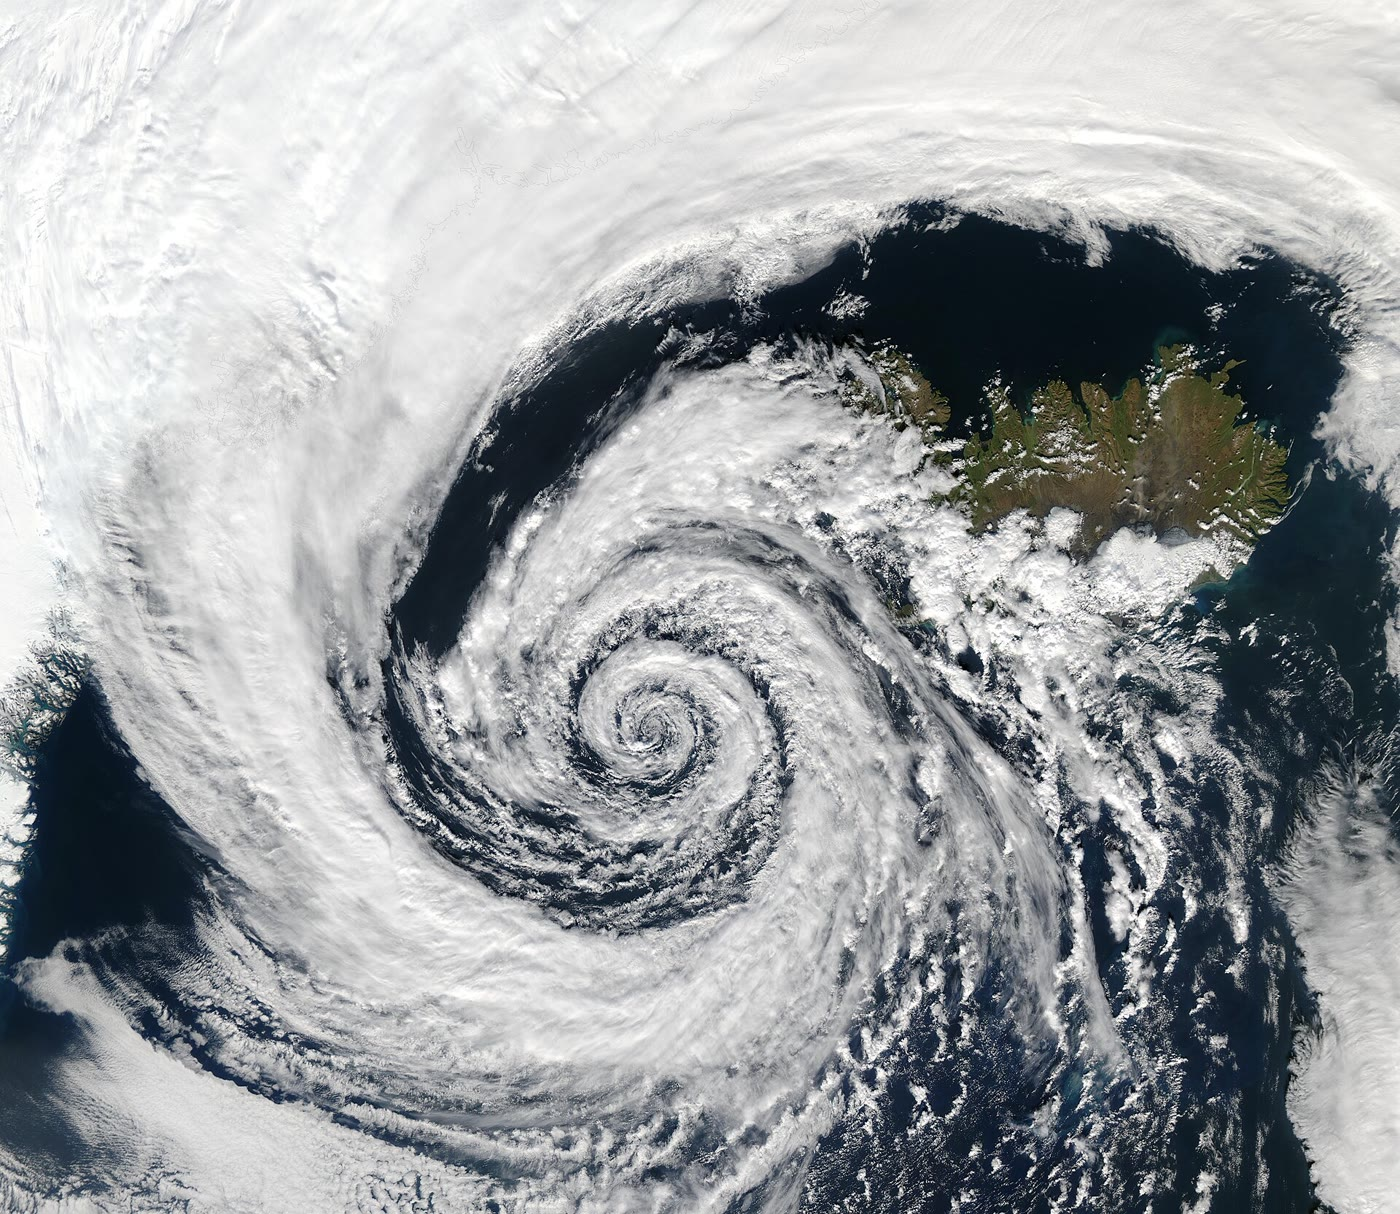
\includegraphics[width=0.58\linewidth]{images/book4/b2-22-iceland-low.jpg}
\par\smallskip{\small Een diepe depressie voor de zuidwestkust van IJsland, 4 september 2003, gezien door
het MODIS-instrument van NASA's satelliet Aqua: de wolkenbanden spiraliseren naar het centrum. (NASA
Goddard Space Flight Center, MODIS Rapid Response Team, Jacques Descloitres, publiek domein, via
Wikimedia Commons.)}
\end{omfigure}

\section{Straalstromen en Rossby-golven}\label{sec:b2:weather-systems:rossby}

Cyclonen liggen niet willekeurig verspreid. De polaire straalstroom, de snelle kern van de westenwinden boven het
poolfront, hangt samen met de ligging en de beweging van de hoge- en lagedrukgebieden van de middelbare
breedten; hij is het snelst langs zijn windmaxima, de stukken waar zijn windsnelheid piekt, en hij
cirkelt niet als een ring om de pool: hij meandert.
% ledger: nws4:polar-front, nws4:jet-streak

\begin{definition}[Rossby-golf; hoogtetrog en hoogterug]\label{def:b2:weather-systems:rossby}
Een \emph{Rossby-golf}\index{Rossby-golf} is een golf van de westelijke stroming van de hogere troposfeer,
een reeks troggen en ruggen van duizenden kilometers lang met een grote noord--zuidamplitude.
Een \emph{hoogtetrog}\index{hoogtetrog} is een langgerekt gebied van relatief lage
druk in zo'n golf, waar de stroming naar de evenaar buigt; een
\emph{hoogterug}\index{hoogterug} is een langgerekt gebied van relatief hoge druk, waar ze naar
de pool buigt.
\end{definition}
% ledger: nws4:rossby

\omterm{def:b2:weather-systems:rossby}{Rossby-golven} bestaan omdat de Coriolisparameter naar de pool toe groeit. Lucht die poolwaarts wordt geduwd,
treft een grotere $f$ aan en draait, met behoud van haar absolute vorticiteit, terug naar de evenaar; lucht
die naar de evenaar wordt geduwd, draait terug naar de pool. De snelheid waarmee $f$ noordwaarts groeit,
$\beta = \mathrm{d}f/\mathrm{d}y = 2\Omega\cos\varphi/a$ met $a$ de straal van de Aarde, bepaalt
hun snelheid. Boek~5 leidt uit het behoud van vorticiteit de fasesnelheid af van een
golf met golflengte $\lambda$ in een uniforme westenwind $U$:
\[
  c = U - \frac{\beta}{k^2}, \qquad k = \frac{2\pi}{\lambda} .
\]
Neem haar hier aan. Ten opzichte van de lucht beweegt elke \omterm{def:b2:weather-systems:rossby}{Rossby-golf} naar het westen, en hoe langer de golf, hoe
sneller; de wind voert haar naar het oosten. Korte golven worden bijna met de snelheid van de wind naar het oosten gevoerd,
lange drijven traag, staan stil of bewegen zelfs naar het westen.
% ledger: earth:Trot, earth:Rmean

\begin{example}[Drie golven op 45° NB]\label{ex:b2:weather-systems:rossby}
Met $\Omega = \qty{7.292e-5}{s^{-1}}$ (een siderische dag van \qty{23.9345}{h}) en $a =
\qty{6371}{km}$ is $\beta = \qty{1.62e-11}{m^{-1}.s^{-1}}$ op \ang{45}~NB. In een westenwind van
\qty{15}{m/s} heeft een golf van \qty{4000}{km} $\beta/k^2 = \qty{6.6}{m/s}$ en beweegt hij oostwaarts met
\qty{8.4}{m/s}; een van \qty{6000}{km} heeft $\beta/k^2 = \qty{14.8}{m/s}$ en beweegt nauwelijks, met
\qty{0.2}{m/s}; een van \qty{8000}{km} beweegt westwaarts met \qty{11.2}{m/s}.
\end{example}
% ledger: earth:Trot, earth:Rmean

De troggen van de lange golven bewegen traag en blijven lang bestaan; de korte golven die erdoorheen trekken,
kortegolftroggen, wekken stijgende lucht op vóór zich, aan hun oostkant, waar de
druk aan het oppervlak daalt en lagedrukgebieden zich ontwikkelen. Een trog waarvan de as van zuidoost naar noordwest helt,
is vaak een teken van een systeem dat zich ontwikkelt of versterkt.
% ledger: nws4:rossby

\begin{omfigure}
\centering
\begin{tikzpicture}[font=\scriptsize, >=Stealth]
\foreach \lat/\pa in {30/-72, 45/-72, 60/-108} {
  \pgfmathsetmacro{\r}{6.0*tan((90-\lat)/2)}
  \draw[black!25] (0,0) circle (\r);
  \node[black!50, fill=white, inner sep=1pt] at (\pa:\r) {\ang{\lat}~NB};
}
\fill (0,0) circle (0.6mm);
\node[anchor=north, black!60] at (0,-0.08) {Noordpool};
\draw[ocBlue, very thick, smooth, samples=241, domain=0:360]
  plot ({6.0*tan((90-(47+11*cos(5*\x)))/2)*cos(\x)}, {6.0*tan((90-(47+11*cos(5*\x)))/2)*sin(\x)});
\foreach \a in {18, 90, 162, 234, 306} {
  \pgfmathsetmacro{\ra}{6.0*tan((90-(47+11*cos(5*\a)))/2)}
  \pgfmathsetmacro{\rb}{6.0*tan((90-(47+11*cos(5*(\a+2))))/2)}
  \draw[ocBlue, very thick, -{Stealth[length=2.6mm]}] (\a:\ra) -- (\a+2:\rb);
}
\pgfmathsetmacro{\rt}{6.0*tan((90-36)/2)}
\node[anchor=216, ocRed!80!black, inner sep=2pt] at (36:\rt) {trog};
\node[anchor=0, ocRed!80!black, inner sep=2pt] at (180:\rt) {trog};
\pgfmathsetmacro{\rr}{6.0*tan((90-58)/2)}
\node[anchor=72, ocRed!80!black, inner sep=3pt] at (72:\rr) {rug};
\end{tikzpicture}
\par\smallskip{\small \omterm{def:b2:weather-systems:rossby}{Rossby-golven} in de straalstroom, gezien van boven de Noordpool (schematisch):
vijf golven rond het halfrond, met troggen die naar de evenaar reiken en ruggen naar de
pool. De straalstroom stroomt oostwaarts, tegen de klok in gezien van boven de pool (pijlen).
Breedtecirkels getekend zoals op een polaire stereografische kaart.}
\end{omfigure}
% ledger: nws4:rossby

Soms houdt het patroon helemaal op met bewegen.

\begin{definition}[Atmosferische blokkering]\label{def:b2:weather-systems:blocking}
\emph{Atmosferische blokkering}\index{atmosferische blokkering} is een groot, aanhoudend en bijna
stationair hogedrukgebied, soms gepaard met een lagedrukgebied, dat de normale oostwaartse
stroming van de straalstroom onderbreekt. Methoden om blokkades op te sporen eisen bijna allemaal dat ze minstens vijf
dagen duren.
\end{definition}
% ledger: wang26:blocking

Een blokkade buigt de straalstroom en de cyclonen eromheen af en houdt dagenlang hetzelfde weer boven hetzelfde
gebied: blokkades brengen hittegolven, droogten, natuurbranden, koudegolven en overstromingen naar de
middelbare breedten. Eind juni en begin juli 2021 leidde een sterke blokkade tot de hittegolf in het
noordwesten van Noord-Amerika aan de Stille Oceaan, die meer dan duizend doden eiste. De fysische
processen achter blokkering zijn nog steeds slecht begrepen, en numerieke modellen hebben moeite om
weer te geven hoe vaak blokkades voorkomen en hoe lang ze duren.
% ledger: wang26:blocking, wang26:gaps

\section{Tropische cyclonen}\label{sec:b2:weather-systems:tropical}

Tropische cyclonen hebben geen fronten en geen temperatuurcontrast om zich mee te voeden. Ze halen hun energie
uit de warme oceaan, via de latente warmte van het water dat ze verdampen, zoals \cref{ch:b2:atmospheric-thermodynamics}
die mat. Zes voorwaarden bevorderen hun ontstaan: oceaanwater van minstens \qty{26.5}{\celsius}
over een diepte van de orde van \qty{50}{m}; een atmosfeer die met de hoogte snel genoeg afkoelt om
onstabiel te zijn voor vochtige convectie; een vochtige middentroposfeer, rond \qty{5}{km}; een afstand van
minstens ongeveer \qty{500}{km} tot de evenaar, zodat de corioliskracht het lagedrukgebied in
evenwicht kan houden; een reeds bestaande verstoring dicht bij het oppervlak; en zwakke verticale windschering, onder ongeveer
\qty{10}{m/s} tussen het oppervlak en de hogere troposfeer. Ze zijn nodig maar niet
voldoende: veel verstoringen die eraan voldoen, ontwikkelen zich nooit.
% ledger: aoml:tc-genesis

Eenmaal gevormd is een tropische cycloon een warmtemotor. Lucht spiraliseert boven zee naar binnen bij bijna
constante temperatuur en neemt warmte en vocht op uit de oceaan; in de oogwand stijgt ze
adiabatisch op; in de uitstroming dicht bij de tropopauze verliest ze warmte door straling bij een lage,
bijna constante temperatuur; en ze daalt weer ver van het centrum, waarmee een cyclus wordt voltooid die
op die van Carnot lijkt. De arbeid van de cyclus drijft de winden aan tegen de wrijving van het
zeeoppervlak.
% ledger: gilford21:pi

\begin{omfigure}
\centering
\begin{tikzpicture}[font=\scriptsize, >=Stealth, x=1cm, y=1cm]
% sea and axis
\fill[ocBlue!12] (0,-0.35) rectangle (12.5,0);
\draw[thick, ocBlue!70!black] (0,0) -- (12.5,0);
\node[anchor=north west, ocBlue!70!black] at (8.6,-0.02) {warme zee, $T_s$};
\draw[dashed, black!50] (0,-0.35) -- (0,4.9);
\node[anchor=south, black!60] at (0,4.9) {centrum};
% eyewall cloud and outflow cloud
\fill[black!14, draw=black!40] (0.9,0.25) .. controls (0.7,1.8) and (0.75,3.3) .. (0.95,4.2)
  .. controls (3.5,4.55) and (7.0,4.45) .. (9.5,4.2) .. controls (7.0,3.9) and (3.6,3.85)
  .. (2.1,3.7) .. controls (1.95,2.6) and (1.9,1.4) .. (2.0,0.25) -- cycle;
\node[black!60] at (0.45,2.0) [rotate=90] {oog};
\draw[black!50] (1.9,1.1) -- (2.45,1.1) node[anchor=west, black!70] {wolk van de oogwand};
% the cycle
\draw[->, very thick, ocRed] (11.4,0.3) -- (2.3,0.3);
\draw[->, very thick, ocRed] (1.45,0.45) .. controls (1.4,1.6) and (1.45,3.0) .. (1.75,4.0);
\draw[->, very thick, ocBlue] (2.2,4.25) -- (11.2,4.25);
\draw[->, very thick, ocBlue] (11.6,4.05) .. controls (11.75,2.8) and (11.75,1.5) .. (11.6,0.45);
\fill (11.6,0.3) circle (0.7mm) node[right=2pt] {A};
\fill (1.45,0.3) circle (0.7mm) node[left=2pt] {B};
\fill (1.8,4.25) circle (0.7mm) node[above left=1pt] {C};
\fill (11.6,4.25) circle (0.7mm) node[above right=1pt] {D};
\node[anchor=south, align=center] at (6.5,0.35) {A$\to$B: instroming bij ongeveer $T_s$,
  opname van warmte en vocht};
\node[anchor=west, align=left] at (2.25,2.3) {B$\to$C: stijgt in de oogwand,\\zonder
  warmte-uitwisseling (natte adiabaat)};
\node[anchor=south, align=center] at (6.5,4.62) {C$\to$D: uitstroming bij de tropopauze bij ongeveer
  $T_o$, warmteverlies door straling};
\node[anchor=east, align=right] at (11.45,2.3) {D$\to$A: daalt ver\\van het centrum};
\end{tikzpicture}
\par\smallskip{\small De warmtemotor van een tropische cycloon, een verticale doorsnede van het centrum
naar buiten (schematisch, niet op schaal): warmte wordt opgenomen bij de temperatuur van het zeeoppervlak
(A$\to$B) en afgestaan bij de veel lagere temperatuur van de uitstroming (C$\to$D), zoals in een
carnotcyclus.}
\end{omfigure}
% ledger: gilford21:pi

\begin{proposition}[Potentiële intensiteit]\label{prop:b2:weather-systems:pi}
\index{potentiële intensiteit}
De \emph{\omterm{prop:b2:weather-systems:pi}{potentiële intensiteit}} van een tropische cycloon, de maximale windsnelheid dicht bij het oppervlak die
de oceaan en de atmosfeer eromheen kunnen onderhouden, wordt bij benadering gegeven door
\[
  V_{\max}^2 = \frac{C_k}{C_D}\,\frac{T_s - T_o}{T_o}\,\bigl(h_o^* - h^*\bigr),
\]
waarin $T_s$ de temperatuur van het zeeoppervlak is, $T_o$ de temperatuur van de uitstroming, $C_k/C_D$
de verhouding van de uitwisselingscoëfficiënten van enthalpie en impuls tussen de zee en de lucht,
meestal op 0.9 gesteld, en $h_o^* - h^*$ het overschot van $c_pT + gz + Lq$ bij verzadiging aan het
zeeoppervlak boven zijn verzadigingswaarde in de lucht boven de grenslaag (aangenomen).
\end{proposition}
% ledger: gilford21:pi

De fractie $(T_s - T_o)/T_o$ is niet het carnotrendement $(T_s - T_o)/T_s$ van de
natuurkundeboeken: ze is groter met de factor $T_s/T_o$, omdat de wrijving die de arbeid dissipeert, de
instromende lucht dicht bij het zeeoppervlak verwarmt, en die warmte door de motor opnieuw wordt gebruikt. De laatste
factor is de brandstof. In een tropische atmosfeer waarvan de temperatuur de \omterm{def:b2:atmospheric-thermodynamics:moist-adiabat}{natte adiabaat} van haar
grenslaaglucht volgt, is $h^*$ de waarde van $c_pT + gz + Lq$ in die lucht, en meet $h_o^* - h^*$
hoe ver de lucht boven zee van verzadiging bij de temperatuur van de zee af is:
\[
  h_o^* - h^* \approx c_p\,(T_s - T_a) + L\,(q_s^* - q_a),
\]
met $T_a$ en $q_a$ de temperatuur en de \omterm{def:b2:atmospheric-thermodynamics:moist-air}{specifieke vochtigheid} van de lucht dicht bij het oppervlak en
$q_s^*$ de verzadigde \omterm{def:b2:atmospheric-thermodynamics:moist-air}{specifieke vochtigheid} bij de temperatuur van het zeeoppervlak.
% ledger: gilford21:pi

\begin{example}[Een potentiële intensiteit]\label{ex:b2:weather-systems:pi}
Boven een zee van \qty{29}{\celsius} heeft de lucht bij \qty{1015}{hPa} een temperatuur van \qty{28}{\celsius} met een
relatieve vochtigheid van \qty{80}{\percent}, en de uitstroming heeft \qty{200}{K}, een typisch
jaargemiddelde boven de warme tropische oceanen. Volgens \cref{prop:b2:atmospheric-thermodynamics:es,prop:b2:atmospheric-thermodynamics:humidity}
is $e_s(\qty{29}{\celsius}) = \qty{41.0}{hPa}$, dus $q_s^* = \qty{25.5}{g/kg}$, en de lucht, met
$e = 0.8 \times \qty{38.7}{hPa}$, heeft $q_a = \qty{19.2}{g/kg}$. Dan is $h_o^* - h^* = 1004.5 \times
1 + 2.501 \times 10^6 \times 0.0063 = \qty{16.8}{kJ/kg}$, is de factor $(T_s - T_o)/T_o$ gelijk aan
$(302.15 - 200)/200 = 0.511$, en is $V_{\max} = \sqrt{0.9 \times 0.511 \times 16\,800} =
\qty{88}{m/s}$.
\end{example}
% ledger: gilford21:pi

De sterkste stormen komen dicht bij zulke waarden: de top van de schaal van Saffir--Simpson, categorie
5, begint bij \qty{70}{m/s}, en vijf recente stormen hebben \qty{86}{m/s} overschreden. De meeste stormen
bereiken zelden hun \omterm{prop:b2:weather-systems:pi}{potentiële intensiteit}: echte stormen zijn zelden in de stationaire toestand die de theorie
aanneemt, en de theorie laat verticale windschering weg, droge lucht die de storm in wordt gezogen en het
dalen van de lucht eromheen, die een storm verzwakken.
% ledger: wk24:scale, gilford21:limits, aoml:tc-weaken

\begin{omfigure}
\centering
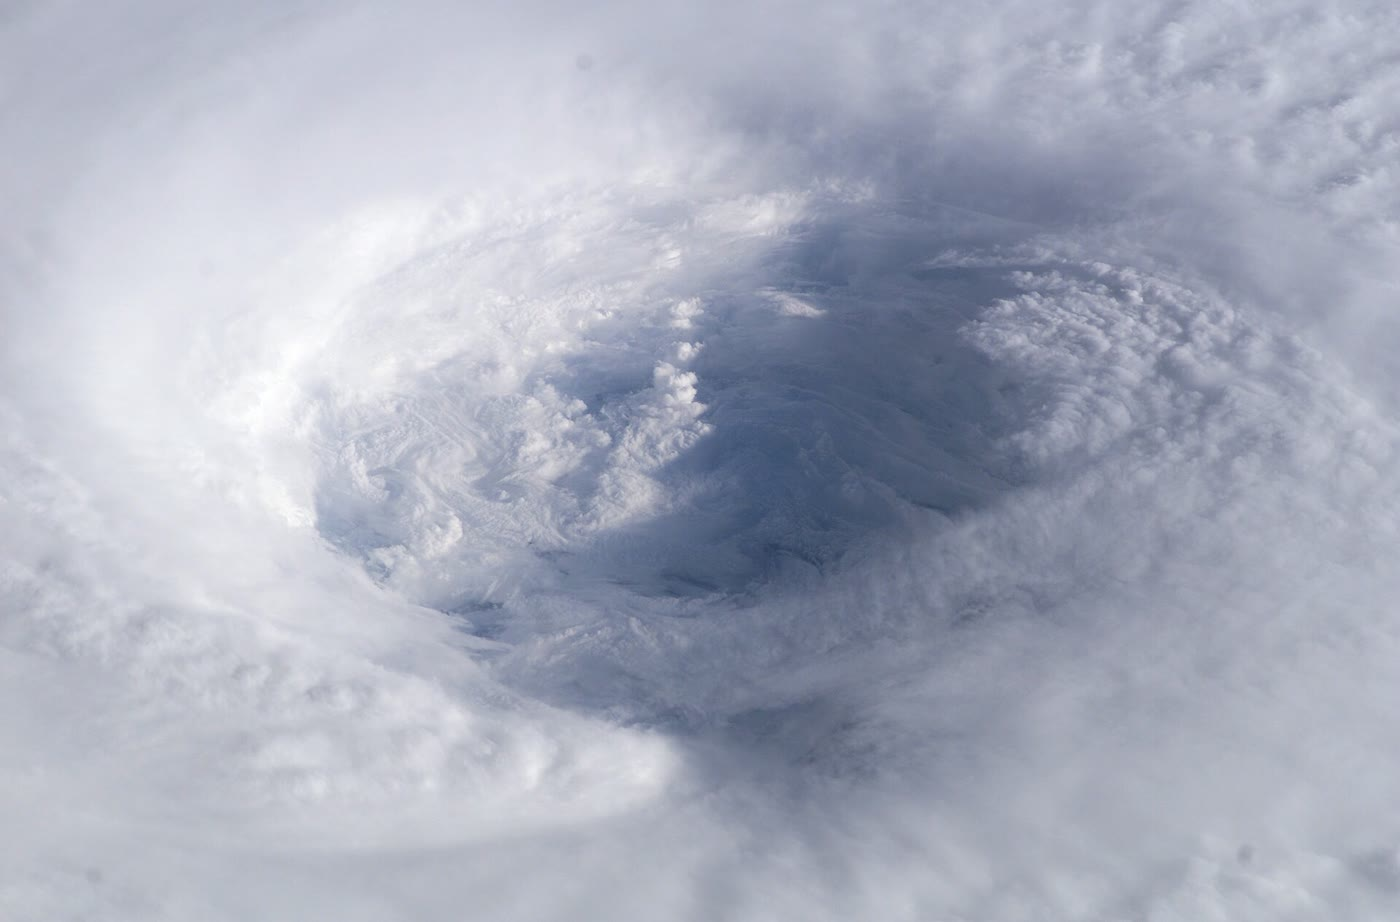
\includegraphics[width=0.62\linewidth]{images/book4/b2-22-isabel-eye.jpg}
\par\smallskip{\small Het oog van orkaan Isabel, 13 september 2003, gefotografeerd vanuit het
internationale ruimtestation ISS: de oogwand valt als een stadion af naar de lage wolken in het oog.
(NASA-astronaut Ed Lu, publiek domein, via Wikimedia Commons.)}
\end{omfigure}

\section{Numerieke weersverwachting}\label{sec:b2:weather-systems:nwp}

\begin{definition}[Numerieke weersverwachting; data-assimilatie; ensembleverwachting; voorspelbaarheidsgrens]\label{def:b2:weather-systems:nwp}
\emph{Numerieke weersverwachting}\index{numerieke weersverwachting} is verwachten met de
computer: de vergelijkingen die de beweging, de energie en het water van de atmosfeer beheersen, worden
vanuit haar waargenomen toestand voorwaarts in de tijd geïntegreerd. \emph{Data-assimilatie}\index{data-assimilatie}
combineert de nieuwste waarnemingen met een kortetermijnverwachting op basis van eerdere
waarnemingen om de beste schatting van de huidige toestand te verkrijgen, de analyse, waarvan de
verwachting uitgaat. Een \emph{ensembleverwachting}\index{ensembleverwachting} is een reeks verwachtingen die
vanuit licht verschillende begintoestanden, en met licht verschillende versies van het model, wordt gedraaid om
het bereik van het mogelijke weer en de waarschijnlijkheid ervan te tonen. De
\emph{voorspelbaarheidsgrens}\index{voorspelbaarheidsgrens} is de tijd waarna een verwachting van de toestand van het
weer niet beter is dan een gok op grond van het klimaat, omdat de fouten in de begintoestand zijn
gegroeid tot ze even groot zijn als de verschillen tussen twee willekeurige toestanden van de atmosfeer.
\end{definition}
% ledger: nws4:nwp, ecmwf4:da, ecmwf4:ens-fs, krish19:predictability

De eerste numerieke verwachting werd in 1950 berekend op ENIAC, een van de eerste elektronische
computers. Een mondiaal model verdeelt de atmosfeer vandaag in een rooster van cellen van enkele kilometers
breed en gaat uit van een analyse die waarnemingen samenvoegt van weerstations, vliegtuigen,
radiosondes, schepen, boeien en vooral satellieten, die de grootste bijdrage leveren aan de
kwaliteit van mondiale verwachtingen. In één groot verwachtingscentrum heeft het ensemble
51 leden, een controlerun en 50 verstoorde runs, met een resolutie van ongeveer \qty{9}{km}, twee keer
per dag gedraaid tot 15 dagen vooruit.
% ledger: krish19:predictability, ecmwf4:da, ecmwf4:ens

Waarom een verwachting verstoren die vanuit de beste analyse zou kunnen starten? Omdat de atmosfeer
chaotisch is, gevoelig voor haar begintoestand. Een systeem van drie variabelen, gepubliceerd in 1963, toont het
op de kleinste schaal.

\begin{proposition}[Het Lorenz-systeem]\label{prop:b2:weather-systems:lorenz}
Het systeem
\[
  \dot x = \sigma(y - x), \qquad \dot y = x(r - z) - y, \qquad \dot z = xy - bz,
\]
met $\sigma = 10$, $r = 28$ en $b = 8/3$, heeft de volgende eigenschappen.
\begin{enumerate}
  \item Zijn vaste punten zijn de oorsprong en $C_\pm = \bigl(\pm\sqrt{b(r - 1)}, \pm\sqrt{b(r - 1)},
        r - 1\bigr) = (\pm 8.49, \pm 8.49, 27)$.
  \item Elk volume in zijn faseruimte krimpt als $\mathrm{e}^{-(\sigma + 1 + b)t}$: zijn
        banen eindigen op een verzameling met volume nul, de attractor.
  \item Op de attractor lopen twee banen die op een kleine afstand $\delta_0$ van elkaar beginnen,
        gemiddeld uiteen als $\delta(t) \approx \delta_0\,\mathrm{e}^{\lambda t}$, met $\lambda =
        0.906$, tot $\delta$ de grootte van de attractor bereikt (berekend, aangenomen). Kleine
        fouten verdubbelen elke $\ln 2/\lambda = 0.77$ tijdseenheden.
\end{enumerate}
\end{proposition}
% ledger: nolitia22:lorenz

\begin{proof}[Bewijs van 1 en 2]
In een vast punt is $y = x$ volgens de eerste vergelijking; de derde geeft $z = x^2/b$; de tweede
wordt $x(r - 1 - x^2/b) = 0$, dus $x = 0$ of $x^2 = b(r - 1) = 72$. De divergentie van het
vectorveld is $\partial_x\dot x + \partial_y\dot y + \partial_z\dot z = -\sigma - 1 - b$, een
constante, en volgens de divergentiestelling gehoorzaamt een volume $V$ dat door de stroming wordt meegevoerd aan $\dot V =
-(\sigma + 1 + b)V$.
\end{proof}

De figuren tonen wat de propositie betekent. Twee runs die \num{e-5} uit elkaar beginnen, volgen elkaar
zo'n vijftien tijdseenheden, en gaan dan definitief uiteen: elk ziet er nog uit als een plausibele
baan van het systeem, maar het is niet langer dezelfde baan. Gemiddeld over 200 paren
runs die \num{e-8} uit elkaar zijn gestart, groeit de afstand exponentieel met de snelheid $\lambda$, een rechte
lijn op een logaritmische schaal, tot ze verzadigt op de grootte van de attractor. Wat de
beginfout ook is, ze bereikt die grootte: een kleinere beginfout stelt het moment alleen uit, met
$\ln 10/\lambda = 2.5$ tijdseenheden per vertienvoudigde verkleining.
% ledger: nolitia22:lorenz

\begin{omfigure}
\centering
% figdata/bachelor-2/weather.py parts traj, butterfly
\begin{tikzpicture}
\begin{groupplot}[group style={group size=2 by 1, horizontal sep=1.5cm},
  tick label style={font=\scriptsize}, label style={font=\small}]
\nextgroupplot[width=0.58\linewidth, height=5.0cm, xmin=0, xmax=30, ymin=-22, ymax=22,
  xlabel={tijd}, ylabel={$x$}, legend style={font=\scriptsize, at={(0.5,1.02)},
  anchor=south, draw=none, legend columns=2, /tikz/every even column/.append style={column
  sep=0.4cm}}, legend cell align=left]
\addplot[ocBlue, thin] table[x=t, y=x1] {figdata/out/bachelor-2-weather-traj.dat};
\addlegendentry{run 1}
\addplot[ocRed, thin, densely dashed] table[x=t, y=x2] {figdata/out/bachelor-2-weather-traj.dat};
\addlegendentry{run 2, \num{e-5} ernaast gestart}
\nextgroupplot[width=0.4\linewidth, height=5.0cm, xmin=-22, xmax=22, ymin=0, ymax=52,
  xlabel={$x$}, ylabel={$z$}]
\addplot[black!70, very thin] table[x=x, y=z] {figdata/out/bachelor-2-weather-butterfly.dat};
\addplot[only marks, mark=*, mark size=1.3pt, ocRed] coordinates {(8.485,27) (-8.485,27)};
\end{groupplot}
\end{tikzpicture}
\par\smallskip{\small Het Lorenz-systeem ($\sigma = 10$, $r = 28$, $b = 8/3$), geïntegreerd met de
methode van Runge--Kutta met een tijdstap van 0.01. Links: twee runs die \num{e-5} uit elkaar in $x$
op de attractor beginnen. Rechts: één run over 40 tijdseenheden, gezien langs $y$, met de vaste punten
$C_\pm$ (rood).}
\end{omfigure}
% ledger: nolitia22:lorenz

\begin{omfigure}
\centering
% figdata/bachelor-2/weather.py part growth
\begin{tikzpicture}
\begin{axis}[width=0.72\linewidth, height=5.6cm, xmin=0, xmax=30, ymode=log, ymin=1e-9,
  ymax=1e3, ytick={1e-9,1e-7,1e-5,1e-3,1e-1,1e1,1e3}, xlabel={tijd}, ylabel={afstand tussen de runs}, tick label style={font=\scriptsize},
  label style={font=\small}, legend style={font=\scriptsize, at={(0.02,0.98)}, anchor=north west,
  draw=none, fill=none}, legend cell align=left, unbounded coords=discard, grid=major,
  grid style={black!8}]
\addplot[ocBlue, line width=1.6pt, opacity=0.55] table[x=t, y expr=10^\thisrow{log10d}]
  {figdata/out/bachelor-2-weather-growth.dat};
\addlegendentry{gemiddelde van 200 paren (meetkundig)}
\addplot[black, densely dashed, thin] table[x=t, y expr=10^\thisrow{fit}]
  {figdata/out/bachelor-2-weather-growth.dat};
\addlegendentry{aangepaste exponentiële functie, $t = 2$ tot 16}
\end{axis}
\end{tikzpicture}
\par\smallskip{\small Groei van de afstand tussen paren runs van het Lorenz-systeem die
\num{e-8} uit elkaar zijn gestart. De aangepaste lijn stijgt met een factor tien per 2.57 tijdseenheden, een snelheid van 0.897;
de grootste Lyapunov-exponent, berekend door één paar over 2000 tijdseenheden te hernormaliseren, is
0.909, tegen 0.906 gepubliceerd. De groei stopt bij de grootte van de attractor.}
\end{omfigure}
% ledger: nolitia22:lorenz

De atmosfeer gedraagt zich op dezelfde manier, met veel meer variabelen en met fouten die met
verschillende snelheden op verschillende schalen groeien. Uit de verwachtingen van de jaren 1980 bleek dat kleine fouten
in ongeveer 2.4 dagen verdubbelen, en de betrouwbare verwachting van de toestand van het weer houdt op vóór
ongeveer tien dagen. Experimenten die de huidige onzekerheid in de begintoestand verkleinen, met een model dat
perfect wordt verondersteld, vinden dat perfecte beginvoorwaarden slechts vier tot vijf dagen zouden toevoegen, en
dat een verkleining met 90 procent daar al bijna alles van geeft: naarmate de fouten kleiner worden, groeien ze
sneller, door het vrijkomen van latente warmte in convectie, op schalen kleiner dan de verwachting
kan oplossen. De \omterm{def:b2:weather-systems:nwp}{voorspelbaarheidsgrens} van de middelbare breedten ligt rond twee weken. Verwachtingen
winnen ongeveer een dag per decennium omdat betere waarnemingen, assimilatie en modellen ze
dichter bij die grens brengen; ze kunnen haar niet overschrijden.
% ledger: krish19:predictability, selz22:limit, bauer:day-per-decade

Het ensemble maakt hier een instrument van. Zijn leden gaan uit van analyses die ongeveer zoveel
verschillen als de analyse zelf onzeker is; zolang ze overeenstemmen, is de verwachting scherp; wanneer ze
uiteenlopen, moet de verwachting dat zeggen, en ze geeft kansen. Een verwachting heet betrouwbaar wanneer
de gebeurtenissen die ze met een kans van \qty{70}{\percent} aankondigt, in \qty{70}{\percent} van
de gevallen plaatsvinden.
% ledger: ecmwf4:ens-fs

\begin{inthelab}[Een dag in een verwachtingscentrum]
\begin{minipage}[t]{0.54\linewidth}\vspace{0pt}
In een mondiaal verwachtingscentrum draait de dag om twee tijdstippen, 00 en 12 UTC. Waarnemingen die
rond elk tijdstip geldig zijn, komen bij miljoenen binnen, van satellieten, radiosondes, vliegtuigen, schepen,
boeien en weerstations; \omterm{def:b2:weather-systems:nwp}{data-assimilatie} voegt ze samen met de vorige korte verwachting tot
de analyse. De modellen starten vanuit de analyse, het ensemble ook, en de verwachtingen bereiken hun gebruikers
enkele uren later, nadat de supercomputers de 15 dagen vooruit hebben doorgerekend. Weervoorspellers
vergelijken dan de runs, toetsen ze aan de nieuwste waarnemingen en de satellietbeelden, volgen
de cyclonen en de fronten, en zetten de kansen van het ensemble om in waarschuwingen en
verwachtingen.
\end{minipage}\hfill
\begin{minipage}[t]{0.42\linewidth}\vspace{0pt}
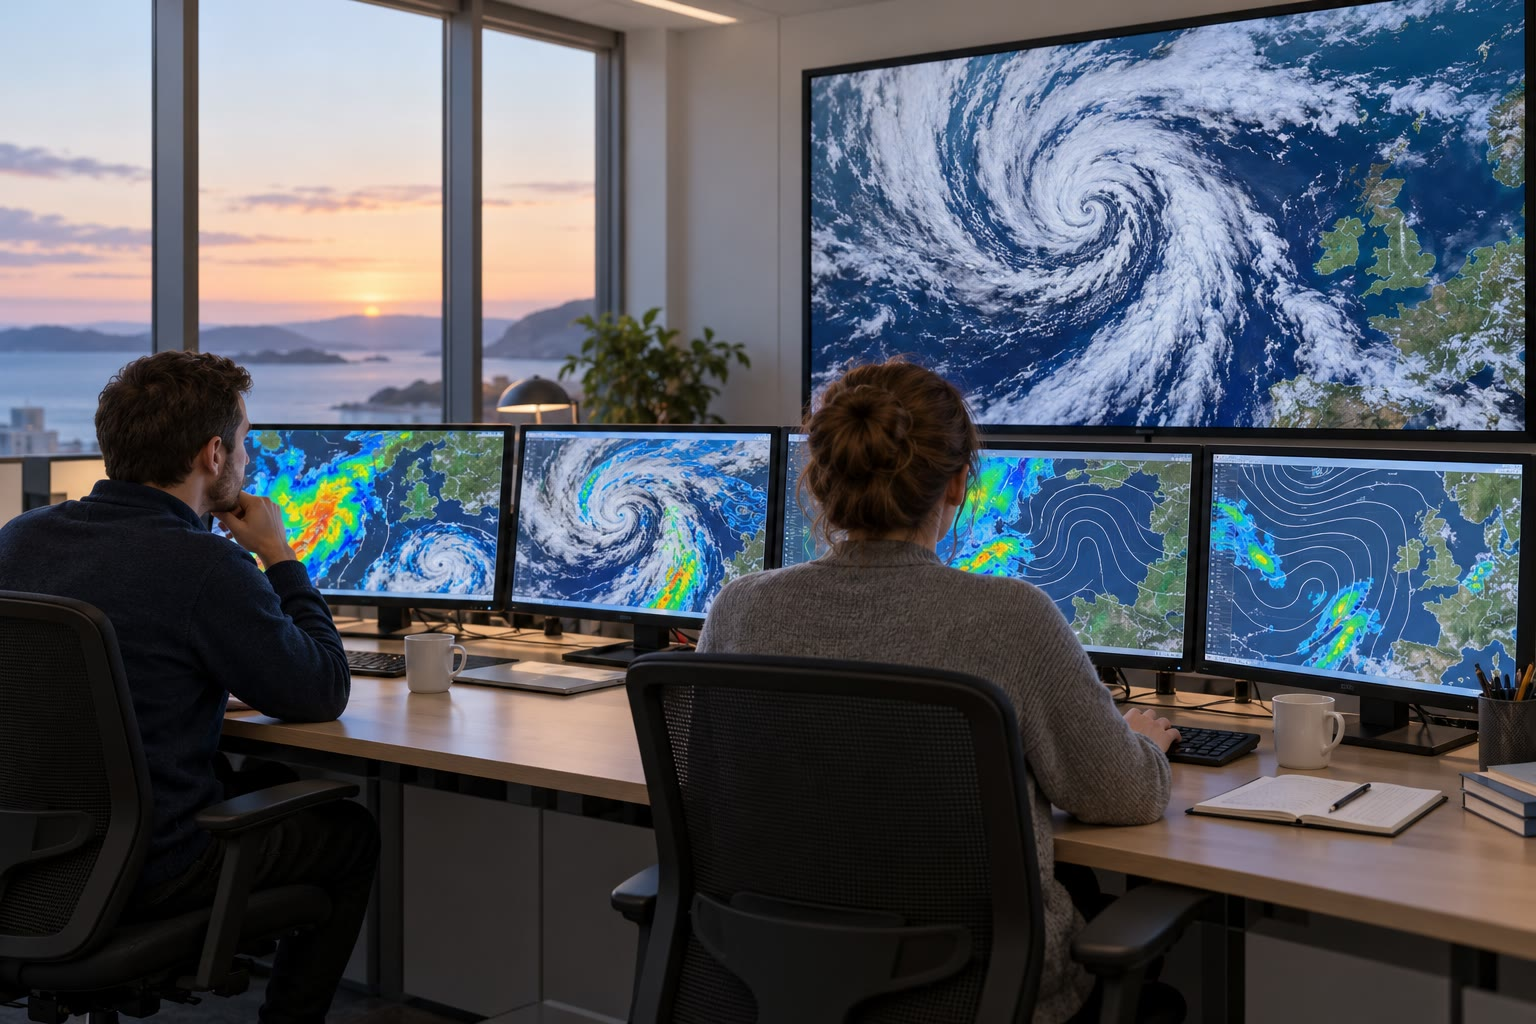
\includegraphics[width=\linewidth]{images/book4/ai/b2-forecast-office.jpg}

{\scriptsize Weervoorspellers aan het werk voor satellietbeelden en modelkaarten
(door AI gegenereerde illustratie).}
\end{minipage}
% ledger: ecmwf4:ens, ecmwf4:da, mo:how-forecasts
\end{inthelab}

\section*{Oefeningen}\label{sec:b2:weather-systems:exercises}

Gegevens voor de oefeningen, tenzij anders vermeld: $\Omega = \qty{7.292e-5}{s^{-1}}$, $a =
\qty{6371}{km}$, $g = \qty{9.81}{m.s^{-2}}$, $c_p = \qty{1004.5}{J.kg^{-1}.K^{-1}}$, $L =
\qty{2.501e6}{J/kg}$, en de verzadigingsdampdruk uit de oefeningen van
\cref{ch:b2:atmospheric-thermodynamics}.
% ledger: earth:Trot, earth:Rmean

\begin{exercise}[$\star$]\label{exo:b2:weather-systems:1}
Op \ang{50}~NB scheidt een koufront lucht van \qty{275}{K} van lucht van \qty{281}{K}, en de wind
erlangs verandert met \qty{15}{m/s}. (a) Bereken $f$. (b) Bereken de helling van het \omterm{def:b2:weather-systems:fronts}{frontvlak},
als 1 op $N$. (c) Hoe ver achter het front aan de grond bereikt het \omterm{def:b2:weather-systems:fronts}{frontvlak}
\qty{1}{km}? (d) Wat gebeurt er met de helling als het temperatuurcontrast verdubbelt bij dezelfde
windsprong?
\end{exercise}

\begin{exercise}[$\star$]\label{exo:b2:weather-systems:2}
Een warm \omterm{def:b2:weather-systems:fronts}{frontvlak} stijgt met 1 op 150 en beweegt met \qty{25}{km/h}. (a) Hoe ver vóór het
front aan de grond ligt het \omterm{def:b2:weather-systems:fronts}{frontvlak} op \qty{6}{km} hoogte? (b) Een waarnemer ziet daar hoge bewolking
op ontstaan. Hoe lang daarna bereikt het front de waarnemer? (c) Beschrijf de opeenvolging van
wolken die de waarnemer intussen ziet.
\end{exercise}
% ledger: ucar:warm-front

\begin{exercise}[$\star$]\label{exo:b2:weather-systems:3}
Op een kaart van het noordelijk halfrond (a) loopt een lijn met blauwe driehoeken aan haar zuidoostkant naar het zuidwesten
vanuit een lagedrukgebied; (b) loopt een lijn met rode halve cirkels aan haar noordkant naar het oosten vanuit hetzelfde lagedrukgebied; (c) loopt een
paarse lijn met beide symbolen van een ander lagedrukgebied naar een punt waar twee andere fronten beginnen;
(d) wisselt een lijn blauwe driehoeken aan haar zuidkant af met rode halve cirkels aan haar noordkant.
Benoem elk front, zeg waar de koude lucht is en welke kant elk op beweegt.
\end{exercise}
% ledger: ucar4:stationary-occluded, nws4:occluded

\begin{exercise}[$\star$]\label{exo:b2:weather-systems:4}
Op \ang{45}~NB in een westenwind van \qty{12}{m/s}: (a) bereken $\beta$. (b) Bereken de fasesnelheid
van golven van \qty{4000}{km} en \qty{8000}{km}. (c) Welke kant beweegt elk op, en hoe ver in een
dag?
\end{exercise}

\begin{exercise}[$\star\star$]\label{exo:b2:weather-systems:5}
(a) Toon aan dat een \omterm{def:b2:weather-systems:rossby}{Rossby-golf} in een westenwind $U$ stilstaat wanneer $\lambda = 2\pi\sqrt{U/\beta}$.
(b) Bereken haar op \ang{45}~NB voor $U = \qty{12}{m/s}$. (c) Hoeveel zulke golven passen er rond de
breedtecirkel? (d) Waarom zou een sterkere westenwind minder, langere stilstaande golven bevorderen?
\end{exercise}

\begin{exercise}[$\star\star$]\label{exo:b2:weather-systems:6}
Voor het Lorenz-systeem: (a) controleer dat $C_+$ een vast punt is door daar de drie afgeleiden
te berekenen. (b) Met welke factor krimpt een klein volume van de faseruimte in één tijdseenheid? (c) Waarom
verhindert dit niet dat twee naburige banen uiteenlopen?
\end{exercise}

\begin{exercise}[$\star\star$]\label{exo:b2:weather-systems:7}
Neem $\lambda = 0.906$ voor het Lorenz-systeem en een attractor met grootte 10. (a) Bereken de
verdubbelingstijd van kleine fouten. (b) Hoe lang doet een fout van \num{e-8} erover om de grootte van
de attractor te bereiken? (c) Hoeveel stelt een duizendmaal kleinere beginfout dat moment uit? Welke
fractie van de tijd uit (b) is dat?
\end{exercise}
% ledger: nolitia22:lorenz

\begin{exercise}[$\star\star$]\label{exo:b2:weather-systems:8}
Een zee van \qty{303}{K} heeft een uitstroming van \qty{195}{K}; het onevenwicht is $h_o^* - h^* =
\qty{15}{kJ/kg}$ en $C_k/C_D = 0.9$. (a) Bereken de \omterm{prop:b2:weather-systems:pi}{potentiële intensiteit}. (b) Vergelijk haar met
de drempel van categorie 5 en met de snelste recente stormen. (c) Waarom bereiken de meeste stormen
haar niet?
\end{exercise}
% ledger: gilford21:pi, wk24:scale

\begin{exercise}[$\star\star$]\label{exo:b2:weather-systems:9}
Voor de storm van \cref{exo:b2:weather-systems:8}: (a) bereken het carnotrendement van een motor
die werkt tussen het zeeoppervlak en de uitstroming. (b) Bereken de factor $(T_s - T_o)/T_o$ van
\cref{prop:b2:weather-systems:pi} en de verhouding van de twee. (c) Verklaar het verschil.
\end{exercise}
% ledger: gilford21:pi

\begin{exercise}[$\star\star\star$]\label{exo:b2:weather-systems:10}
(a) Leid \cref{prop:b2:weather-systems:slope} opnieuw af met exacte dichtheden, en toon aan dat
de koude lucht onder moet liggen. (b) Over een frontale zone van \qty{50}{km} breed op \ang{45}~NB verandert de wind
langs het front met \qty{10}{m/s}. Bereken de relatieve vorticiteit van de zone en vergelijk
die met $f$. (c) Is de zone cyclonaal of anticyclonaal?
\end{exercise}

\begin{exercise}[$\star\star\star$]\label{exo:b2:weather-systems:11}
Stel dat verwachtingsfouten elke 2.4 dagen verdubbelen, beginnen bij \qty{0.5}{K} en onbruikbaar zijn bij
\qty{6}{K}. (a) Bepaal de horizon van bruikbare verwachtingen. (b) Met welke factor moet de beginfout
elk decennium krimpen om een dag per decennium te winnen, als het model perfect was? (c) Experimenten vinden dat
een tienmaal kleinere beginfout slechts 4 tot 5 dagen wint. Welke verdubbelingstijd impliceert dat voor
kleine fouten, en wat zegt het over hoe kleine fouten groeien?
\end{exercise}
% ledger: krish19:predictability, selz22:limit, bauer:day-per-decade

\begin{exercise}[$\star\star\star$]\label{exo:b2:weather-systems:12}
Neem \cref{ex:b2:weather-systems:pi} en warm zowel de zee als de lucht \qty{1}{K} op, met
ongewijzigde relatieve vochtigheid en uitstroomtemperatuur. (a) Bereken $q_s^*$, $q_a$ en het
onevenwicht opnieuw. (b) Bereken de \omterm{prop:b2:weather-systems:pi}{potentiële intensiteit} opnieuw. (c) Met hoeveel procent per kelvin
stijgt ze, en welke factor draagt het meest bij?
\end{exercise}
% ledger: gilford21:pi

\begin{problem}[{Weekendprobleem --- Hoe ver vooruit?}]\label{pb:b2:weather-systems:1}
Een verzonnen weerkaart op \ang{50}~NB toont een koufront dat op een stad afkomt, met een
\omterm{def:b2:weather-systems:rossby}{Rossby-golf} in de straalstroom erboven. Het probleem volgt het front, dan de golf, en vraagt dan hoe ver
vooruit iets ervan kan worden verwacht. Gebruik de gegevens van de oefeningen.

\medskip\noindent\textbf{Deel I --- Het front.}
Om 06 UTC ligt het koufront \qty{480}{km} ten westen van de stad, om 12 UTC \qty{390}{km}. Erachter
heeft de lucht \qty{277}{K}, in de warme sector \qty{285}{K}, en de wind langs het front
verandert over het front met \qty{16}{m/s}.
\begin{enumerate}
  \item Bepaal de snelheid van het front.
  \item Hoe laat bereikt het de stad?
  \item Bereken $f$ op \ang{50}~NB.
  \item Bereken de helling van het \omterm{def:b2:weather-systems:fronts}{frontvlak}.
  \item Hoe hoog ligt het \omterm{def:b2:weather-systems:fronts}{frontvlak} boven de stad zes uur nadat het front is gepasseerd?
  \item Hoe lang na de passage bereikt de koude lucht \qty{1.5}{km} boven de stad?
  \item Welk weer ziet de stad wanneer het front passeert, en hoe verandert de druk?
\end{enumerate}

\medskip\noindent\textbf{Deel II --- De golf in de hoogte.}
In de straalstroom erboven waait een westenwind van \qty{20}{m/s} en heeft de golf een golflengte van \qty{5000}{km}.
\begin{enumerate}[resume]
  \item Bereken $\beta$ op \ang{50}~NB.
  \item Bereken $k$ en $\beta/k^2$.
  \item Bepaal de fasesnelheid van de golf.
  \item Hoe ver beweegt een trog in 24 uur?
  \item Bepaal de golflengte die in deze wind zou stilstaan, en hoeveel zulke golven er passen
        rond \ang{50}~NB.
  \item Waar, ten opzichte van de \omterm{def:b2:weather-systems:rossby}{hoogtetrog}, zou de cycloon aan het oppervlak moeten verdiepen?
\end{enumerate}

\medskip\noindent\textbf{Deel III --- Een speelgoedatmosfeer.}
In de figuur van de groei van fouten in het Lorenz-systeem gaat de aangepaste lijn door
ongeveer \num{5e-7} bij $t = 4$ en \num{3.9e-3} bij $t = 14$.
\begin{enumerate}[resume]
  \item Bereken uit deze twee aflezingen de groeisnelheid $\lambda$.
  \item Bereken de verdubbelingstijd.
  \item Vergelijk met de gepubliceerde exponent 0.906.
  \item Waarom houdt de afstand op met groeien, bij ongeveer 15?
  \item Hoeveel later bereikt een tien keer kleinere fout die grootte?
\end{enumerate}

\medskip\noindent\textbf{Deel IV --- Hoe ver vooruit?}
Neem de verdubbelingstijd van 2.4 dagen die voor kleine fouten van de verwachtingen van de jaren 1980 werd gevonden, een
beginfout van \qty{0.1}{\celsius} in de temperatuur op een bepaald niveau, en een verwachting die
onbruikbaar is zodra de fout \qty{3}{\celsius} bereikt.
\begin{enumerate}[resume]
  \item Hoeveel verdubbelingen scheiden de beginfout van de onbruikbare?
  \item Hoeveel dagen kost dat?
  \item Hoeveel dagen zou een halvering van de beginfout opleveren?
  \item Welke horizon zou men vinden met de vroegere schatting van een verdubbelingstijd van 5 dagen?
  \item Moderne experimenten vinden dat een tienmaal kleinere beginfout, en zelfs een perfecte
        begintoestand, slechts 4 tot 5 dagen wint. Waarom suggereert dat dat de schatting van
        vraag 20 optimistisch is?
  \item Samengevat: hoe ver vooruit, in dagen, zou deze verwachting bruikbaar kunnen zijn?
\end{enumerate}
\end{problem}
% ledger: krish19:predictability, selz22:limit, nolitia22:lorenz, ucar:cold-front
